\section{Parser}

Każdy z dokumentów HTML'a musi zawierać znaczniki typowe dla tego formatu, których nie znajdziemy w dokumentach \LaTeX. Są to: \textbf{\textit{html}},
\textbf{\textit{head}} oraz \textbf{\textit{body}}. Jako odpowienik sekcji \textbf{\textit{head}} przyjęliśmy sekcję preambuly w której 
znajdują się między innymi takie polecenia jak \textit{usepackage}. Natomiast jak odpowiednik sekcji \textbf{\textit{body}} odpowiada fragment kodu 
\LaTeX \space objęty poleceniami \textit{begin\{document\}} oraz \textit{end\{document\}}.

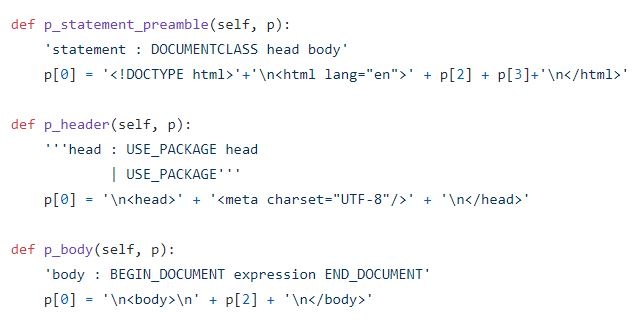
\includegraphics{preamble.JPG}

\subsection{Obsługa tekstu}

\begin{lstlisting}[language={Python}, caption={Gramatyka - tekst}, label={gramatyka-tekst}]
    def p_expression_text(self, p):
        '''expression : TEXT expression
                      | TEXT'''
        if len(p) == 3:
            p[0] = p[1] + " " + p[2]
        else:
            p[0] = p[1]
\end{lstlisting}

\subsection{Formatowanie tekstu}

Nasz translator umożliwia pogrubienie, kursywę, podkreślenie, wyśrodkowanie tekstu oraz utworzenie paragrafu. 
Możliwe jest mieszanie stylów formatowania, np. pogrubienie z podkreśleniem. 
Według nowych zaleceń, do pogrubienia tekstu w HTML'u powinno się stosować znacznik
\textit{$<$strong$>$}, a do kursywy \textit{$<$em$>$}.

\begin{lstlisting}[language={Python}, caption={Formatowanie - pogrubienie, kursywa, podkreślenie, wyśrodkowanie tekstu}, label={gramatyka-pogrubienie-kursywa}]
    def p_expression_bold(self, p):
        '''expression : BOLD LBRACE expression RBRACE expression
                      | BOLD LBRACE expression RBRACE'''
        if len(p) == 6:
            p[0] = '<strong>' + p[3] + '</strong>' + p[5]
        else:
            p[0] = '<strong>' + p[3] + '</strong>'

    def p_expression_italic(self, p):
        '''expression : ITALIC LBRACE expression RBRACE expression
                      | ITALIC LBRACE expression RBRACE'''
        if len(p) == 6:
            p[0] = '<em>' + p[3] + '</em>' + p[5]
        else:
            p[0] = '<em>' + p[3] + '</em>'

    def p_expression_underline(self, p):
        '''expression : UNDERLINE LBRACE expression RBRACE expression
                      | UNDERLINE LBRACE expression RBRACE'''
        if len(p) == 6:
            p[0] = '<u>' + p[3] + '</u>' + p[5]
        else:
            p[0] = '<u>' + p[3] + '</u>'

    def p_expression_centerline(self, p):
        '''expression : CENTERLINE LBRACE expression RBRACE expression
                      | CENTERLINE LBRACE expression RBRACE'''
        if len(p) == 6:
            p[0] = '<center>' + p[3] + '</center>' + p[5]
        else:
            p[0] = '<center>' + p[3] + '</center>'

    def p_expression_paragraph(self, p):
        '''expression : PARAGRAPH LBRACE expression RBRACE expression
                      | PARAGRAPH LBRACE expression RBRACE'''
        if len(p) == 6:
            p[0] = '<p>' + p[3] + '</p>' + p[5]
        else:
            p[0] = '<p>' + p[3] + '</p>'
\end{lstlisting}

Kolejną funkcjonalnością jest możliwość obsługi rozdziałów, sekcji i podsekcji parsując 
znaczniki \textit{chapter}, \textit{section}, \textit{subsection} oraz \textit{subsubsection}.

\begin{lstlisting}[language={Python}, caption={Rozdziały, sekcje i podsekcje}, label={gramatyka-sekcje-podsekcje}]
    def p_expression_chapter(self, p):
        '''expression : CHAPTER LBRACE expression RBRACE expression
                      | CHAPTER LBRACE expression RBRACE'''
        if len(p) == 6:
            p[0] = '<h1>' + p[3] + '</h1>' + p[5]
        else:
            p[0] = '<h1>' + p[3] + '</h1>'

    def p_expression_section(self, p):
        '''expression : SECTION LBRACE expression RBRACE expression
                      | SECTION LBRACE expression RBRACE'''
        if len(p) == 6:
            p[0] = '<h2>' + p[3] + '</h2>' + p[5]
        else:
            p[0] = '<h2>' + p[3] + '</h2>'

    def p_expression_subsection(self, p):
        '''expression : SUBSECTION LBRACE expression RBRACE expression
                      | SUBSECTION LBRACE expression RBRACE'''
        if len(p) == 6:
            p[0] = '<h3>' + p[3] + '</h3>' + p[5]
        else:
            p[0] = '<h3>' + p[3] + '</h3>'

    def p_expression_subsubsection(self, p):
        '''expression : SUBSUBSECTION LBRACE expression RBRACE expression
                      | SUBSUBSECTION LBRACE expression RBRACE'''
        if len(p) == 6:
            p[0] = '<h4>' + p[3] + '</h4>' + p[5]
        else:
            p[0] = '<h4>' + p[3] + '</h4>'
\end{lstlisting}

Przejście do nowej linii (hard break) jest obsłużone poleceniem \textit{newline}.

\begin{lstlisting}[language={Python}, caption={Nowa linia}, label={gramatyka-nowa-linia}]
    def p_expression_newline(self, p):
        '''expression : NEW_LINE expression
                      | NEW_LINE'''
        if len(p) == 3:
            p[0] = '<br/>' + p[2]
        else:
            p[0] = p[1]
\end{lstlisting}

Translator parsuje również znacznik \textit{title} odpowiadający za utworzenie tytułu.

\begin{lstlisting}[language={Python}, caption={Tytuł}, label={gramatyka-tyti}]
    def p_title(self, p):
        'expression : TITLE LBRACE TEXT RBRACE'
        p[0] = '<i>' + p[3] + '</i>'
\end{lstlisting}

\subsection{Tabela}

\subsubsection{Z obramowaniem}

\begin{lstlisting}[language={Python}, caption={Tabela z obramowaniem}, label={gramatyka-tekst}]
    def p_expression_table_bordered(self, p):
        '''expression : BEGIN_TABULAR COLUMN_PATTERN_BORDERED tablerowbordered END_TABULAR expression | BEGIN_TABULAR COLUMN_PATTERN_BORDERED tablerowbordered END_TABULAR'''
        if len(p) == 6:
            p[0] = '<table style="border: 1px solid black; border-collapse: collapse;">' + p[3] + '</table>' + p[5]
        else:
            p[0] = '<table style="border: 1px solid black; border-collapse: collapse;">' + p[3] + '</table>'

    def p_tablerowbordered(self, p):
        '''tablerowbordered : tablecolumnbordered ROW_END tablerowbordered | tablecolumnbordered'''
        if len(p) == 4:
            p[0] = '<tr>' + p[1] + '</tr>' + p[3]
        else:
            p[0] = '<tr>' + p[1] + '</tr>'

    def p_tablecolumnbordered(self, p):
        '''tablecolumnbordered : expression COLUMN_DIVIDER tablecolumnbordered | expression'''
        if len(p) == 4:
            p[0] = '<td style="border: 1px solid black; border-collapse: collapse;">' + p[1] + '</td>' + p[3]
        else:
            p[0] = '<td style="border: 1px solid black; border-collapse: collapse;">' + p[1] + '</td>'
\end{lstlisting}

\subsubsection{Bez obramowania}

\begin{lstlisting}[language={Python}, caption={Tabela bez obramowania}, label={gramatyka-tekst} ]
    def p_expression_table_borderless(self, p):
        '''expression : BEGIN_TABULAR COLUMN_PATTERN_BORDERLESS tablerowborderless END_TABULAR expression | BEGIN_TABULAR COLUMN_PATTERN_BORDERLESS tablerowborderless END_TABULAR'''
        if len(p) == 6:
            p[0] = '<table>' + p[3] + '</table>' + p[5]
        else:
            p[0] = '<table>' + p[3] + '</table>'

    def p_tablerowborderless(self, p):
        '''tablerowborderless : tablecolumnborderless ROW_END tablerowborderless | tablecolumnborderless'''
        if len(p) == 4:
            p[0] = '<tr>' + p[1] + '</tr>' + p[3]
        else:
            p[0] = '<tr>' + p[1] + '</tr>'

    def p_tablecolumnborderless(self, p):
        '''tablecolumnborderless : expression COLUMN_DIVIDER tablecolumnborderless | expression'''
        if len(p) == 4:
            p[0] = '<td>' + p[1] + '</td>' + p[3]
        else:
            p[0] = '<td>' + p[1] + '</td>'
\end{lstlisting}

\subsection{Wyliczenie}

Konstrukcja parsera wyliczeń umożliwia wykonywanie zagnieżdżeń.

\subsubsection{Uporządkowane}

\begin{lstlisting}[language={Python}, caption={Gramatyka - tabela}, label={gramatyka-tekst} ]
    def p_expression_ordered_list(self, p):
        '''expression : BEGIN_OLIST listitems END_OLIST expression
                      | BEGIN_OLIST listitems END_OLIST'''
        if len(p) == 5:
            p[0] = '\n<ol>' + p[2] + '\n</ol>' + p[4]
        else:
            p[0] = '\n<ol>' + p[2] + '\n</ol>'
\end{lstlisting}

\subsubsection{Nieuporządkowane}

\begin{lstlisting}[language={Python}, caption={Gramatyka - tabela}, label={gramatyka-tekst} ]
    def p_expression_unordered_list(self, p):
        '''expression : BEGIN_ULIST listitems END_ULIST expression
                      | BEGIN_ULIST listitems END_ULIST'''
        if len(p) == 5:
            p[0] = '\n<ul>' + p[2] + '\n</ul>' + p[4]
        else:
            p[0] = '\n<ul>' + p[2] + '\n</ul>'
\end{lstlisting}

\subsection{Grafika}

Umieszcznie grafiki jest możliwe dzięki znacznikowi \textit{includegraphics} w \LaTeX, który jest parsowany na znacznik 
\textit{$<$img$>$} w HTML, gdzie atrybut \textit{src} stanowi ścieżka do pliku umieszczona w nawiasach 
wąsatych w dokumencie \LaTeX.

\begin{lstlisting}[language={Python}, caption={Grafika}, label={gramatyka-tekst} ]
    def p_expression_includegraphics(self, p):
        '''expression : INCLUDE_GRAPHICS TEXT LBRACE expression RBRACE expression 
                      | INCLUDE_GRAPHICS LBRACE expression RBRACE expression 
                      | INCLUDE_GRAPHICS LBRACE expression RBRACE'''
        if len(p) == 7:
            attributes = p[2][1:-1]
            p[0] = '''<img src="''' + p[4] + '''"''' + attributes + '''>''' + p[6]
        elif len(p) == 6:
            p[0] = '''<img src="''' + p[3] + '''">''' + p[5]
        else:
            p[0] = '''<img src="''' + p[3] + '''">'''
\end{lstlisting}

\subsection{Hiperłącze}

Zamieszczenie hiperłącza w formacie \LaTeX jest możliwe dzięki znacznikowi \textit{url}, 
zawierającego w nawiasach wąsatych adres do strony.
Parsowanny jest on na HTML'owy znacznik \textit{$<$a$>$} z atrybutem \textit{href} zawierającego adres.

\begin{lstlisting}[language={Python}, caption={Hiperłącze}, label={gramatyka-hiperlacze} ]
    def p_expression_url(self, p):
        '''expression : URL LBRACE expression RBRACE expression
                      | URL LBRACE expression RBRACE'''
        if len(p) == 6:
            p[0] = '<a href=' + p[3] + '>' + p[3] + '</a>' + p[5]
        else:
            p[0] = '<a href=' + p[3] + '>' + p[3] + '</a>'
\end{lstlisting}